% Generated from summary_results.csv.
\begin{figure}[tbp]
\centering
\pgfplotsset{compat=1.18}
\begin{subfigure}{0.245\textwidth}
\centering
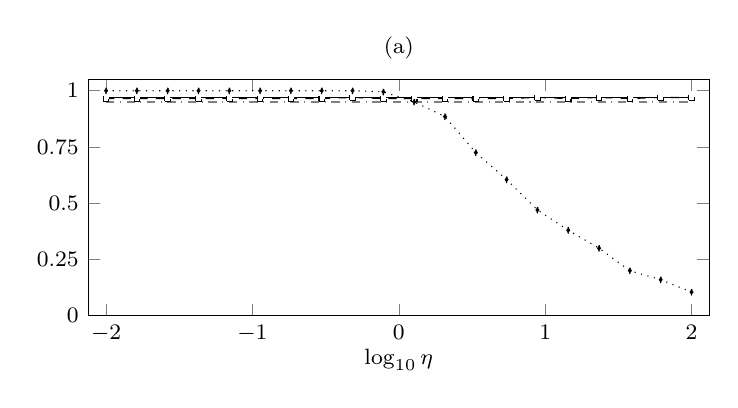
\begin{tikzpicture}
\begin{axis}[
    title={(a)},
    xlabel={$\log_{10}\eta$},
    xmode=log,
    log basis x=10,
    xmin=0.01,
    xmax=100,
    enlarge x limits=0.03,
    xtick={0.01,0.1,1,10,100},
    xticklabels={$-2$, $-1$, $0$, $1$, $2$},
    scaled y ticks=false,
    scale only axis,
    width=0.65\linewidth,
    height=3.0cm,
    mark size=1.0pt,
    font=\footnotesize,
    xlabel style={yshift=1ex},
    title style={yshift=-0.5ex},
    ymin=0,
    ymax=1.05,
    ytick={0,0.25,0.5,0.75,1},
    yticklabel style={/pgf/number format/fixed,/pgf/number format/precision=2},
]
\addplot[gray, dashdotted, mark=none, line width=0.4pt, forget plot]
coordinates
{(0.01,0.95) (100,0.95)}
;
\addplot[black, solid, mark=none]
coordinates
{(0.01,0.97) (0.016237767391887217,0.97) (0.02636650898730358,0.97) (0.04281332398719394,0.97) (0.06951927961775606,0.97) (0.11288378916846889,0.97) (0.18329807108324356,0.97) (0.29763514416313175,0.97) (0.4832930238571752,0.97) (0.7847599703514611,0.97) (1.2742749857031335,0.97) (2.06913808111479,0.97) (3.359818286283781,0.97) (5.455594781168514,0.97) (8.858667904100823,0.97) (14.38449888287663,0.97) (23.357214690901213,0.97) (37.92690190732246,0.97) (61.584821106602604,0.97) (100.0,0.97)}
;
\addplot[black, dashed, mark=square*, mark size=1.0pt, mark options={fill=white}]
coordinates
{(0.01,0.965) (0.016237767391887217,0.965) (0.02636650898730358,0.965) (0.04281332398719394,0.965) (0.06951927961775606,0.965) (0.11288378916846889,0.965) (0.18329807108324356,0.965) (0.29763514416313175,0.965) (0.4832930238571752,0.97) (0.7847599703514611,0.965) (1.2742749857031335,0.965) (2.06913808111479,0.965) (3.359818286283781,0.965) (5.455594781168514,0.965) (8.858667904100823,0.97) (14.38449888287663,0.965) (23.357214690901213,0.97) (37.92690190732246,0.965) (61.584821106602604,0.97) (100.0,0.97)}
;
\addplot[black, dotted, mark=diamond*, mark size=1.0pt]
coordinates
{(0.01,1.0) (0.016237767391887217,1.0) (0.02636650898730358,1.0) (0.04281332398719394,1.0) (0.06951927961775606,1.0) (0.11288378916846889,1.0) (0.18329807108324356,1.0) (0.29763514416313175,1.0) (0.4832930238571752,1.0) (0.7847599703514611,0.995) (1.2742749857031335,0.95) (2.06913808111479,0.885) (3.359818286283781,0.725) (5.455594781168514,0.605) (8.858667904100823,0.47) (14.38449888287663,0.38) (23.357214690901213,0.3) (37.92690190732246,0.2) (61.584821106602604,0.16) (100.0,0.105)}
;
\end{axis}
\end{tikzpicture}
\end{subfigure}%
\hfill
\begin{subfigure}{0.245\textwidth}
\centering
\begin{tikzpicture}
\begin{axis}[
    title={(b)},
    xlabel={$\log_{10}\eta$},
    xmode=log,
    log basis x=10,
    xmin=0.01,
    xmax=100,
    enlarge x limits=0.03,
    xtick={0.01,0.1,1,10,100},
    xticklabels={$-2$, $-1$, $0$, $1$, $2$},
    scaled y ticks=false,
    scale only axis,
    width=0.65\linewidth,
    height=3.0cm,
    mark size=1.0pt,
    font=\footnotesize,
    xlabel style={yshift=1ex},
    title style={yshift=-0.5ex},
    ymin=0,
    enlarge y limits={upper,value=0.04},
    ytick distance=0.5,
    yticklabel style={/pgf/number format/fixed,/pgf/number format/precision=1},
]
\addplot[black, solid, mark=none]
coordinates
{(0.01,0.19331614393643315) (0.016237767391887217,0.19331614393643315) (0.02636650898730358,0.19331614393643315) (0.04281332398719394,0.19331614393643315) (0.06951927961775606,0.19331614393643315) (0.11288378916846889,0.19331614393643315) (0.18329807108324356,0.19331614393643315) (0.29763514416313175,0.19331614393643315) (0.4832930238571752,0.19331614393643315) (0.7847599703514611,0.19331614393643315) (1.2742749857031335,0.19331614393643315) (2.06913808111479,0.19331614393643315) (3.359818286283781,0.19331614393643315) (5.455594781168514,0.19331614393643315) (8.858667904100823,0.19331614393643315) (14.38449888287663,0.19331614393643315) (23.357214690901213,0.19331614393643315) (37.92690190732246,0.19331614393643315) (61.584821106602604,0.19331614393643315) (100.0,0.19331614393643315)}
;
\addplot[black, dashed, mark=square*, mark size=1.0pt, mark options={fill=white}]
coordinates
{(0.01,0.19310675255083773) (0.016237767391887217,0.19311091814928155) (0.02636650898730358,0.19315959867936067) (0.04281332398719394,0.19324076150055472) (0.06951927961775606,0.19327057397640268) (0.11288378916846889,0.19328969435018364) (0.18329807108324356,0.19317614000373962) (0.29763514416313175,0.1932695415415661) (0.4832930238571752,0.19332383031593595) (0.7847599703514611,0.19306820047011372) (1.2742749857031335,0.19333418569435884) (2.06913808111479,0.1933170766826308) (3.359818286283781,0.1932582708612432) (5.455594781168514,0.1932427280378164) (8.858667904100823,0.1931860827903764) (14.38449888287663,0.19331095967647471) (23.357214690901213,0.19326337511128472) (37.92690190732246,0.19322336206195959) (61.584821106602604,0.19332879829150568) (100.0,0.19329282673954473)}
;
\addplot[black, dotted, mark=diamond*, mark size=1.0pt]
coordinates
{(0.01,2.068813050551103) (0.016237767391887217,1.6260394447663418) (0.02636650898730358,1.2765895062545416) (0.04281332398719394,1.001904850120538) (0.06951927961775606,0.786885502959725) (0.11288378916846889,0.6178115969952295) (0.18329807108324356,0.4844986116487134) (0.29763514416313175,0.38051341248460213) (0.4832930238571752,0.2988618957137781) (0.7847599703514611,0.23406607064367135) (1.2742749857031335,0.18397605994995106) (2.06913808111479,0.14428999591533143) (3.359818286283781,0.11323057170661446) (5.455594781168514,0.08889660424553318) (8.858667904100823,0.06970779488910298) (14.38449888287663,0.05472973127596521) (23.357214690901213,0.04296168101215775) (37.92690190732246,0.033709760694856504) (61.584821106602604,0.0264781313752965) (100.0,0.02076771876595599)}
;
\end{axis}
\end{tikzpicture}
\end{subfigure}%
\hfill
\begin{subfigure}{0.245\textwidth}
\centering
\begin{tikzpicture}
\begin{axis}[
    title={(c)},
    xlabel={$\log_{10}\eta$},
    xmode=log,
    log basis x=10,
    xmin=0.01,
    xmax=100,
    enlarge x limits=0.03,
    xtick={0.01,0.1,1,10,100},
    xticklabels={$-2$, $-1$, $0$, $1$, $2$},
    scaled y ticks=false,
    scale only axis,
    width=0.65\linewidth,
    height=3.0cm,
    mark size=1.0pt,
    font=\footnotesize,
    xlabel style={yshift=1ex},
    title style={yshift=-0.5ex},
    enlarge y limits=0.08,
    ytick distance=0.01,
    yticklabel style={/pgf/number format/fixed,/pgf/number format/precision=2},
]
\addplot[gray!60, solid, mark=none, line width=0.3pt, forget plot]
coordinates
{(0.01,0) (100,0)}
;
\addplot[black, solid, mark=none]
coordinates
{(0.01,0.0025387683360829274) (0.016237767391887217,0.0025387683360829274) (0.02636650898730358,0.0025387683360829274) (0.04281332398719394,0.0025387683360829274) (0.06951927961775606,0.0025387683360829274) (0.11288378916846889,0.0025387683360829274) (0.18329807108324356,0.0025387683360829274) (0.29763514416313175,0.0025387683360829274) (0.4832930238571752,0.0025387683360829274) (0.7847599703514611,0.0025387683360829274) (1.2742749857031335,0.0025387683360829274) (2.06913808111479,0.0025387683360829274) (3.359818286283781,0.0025387683360829274) (5.455594781168514,0.0025387683360829274) (8.858667904100823,0.0025387683360829274) (14.38449888287663,0.0025387683360829274) (23.357214690901213,0.0025387683360829274) (37.92690190732246,0.0025387683360829274) (61.584821106602604,0.0025387683360829274) (100.0,0.0025387683360829274)}
;
\addplot[black, dashed, mark=square*, mark size=1.0pt, mark options={fill=white}]
coordinates
{(0.01,0.0025387683360829226) (0.016237767391887217,0.0025387683360829296) (0.02636650898730358,0.0025387683360829244) (0.04281332398719394,0.0025387683360829382) (0.06951927961775606,0.0025387683360829257) (0.11288378916846889,0.002538768336082924) (0.18329807108324356,0.002538768336082932) (0.29763514416313175,0.0025387683360829283) (0.4832930238571752,0.0025387683360829265) (0.7847599703514611,0.0025387683360829343) (1.2742749857031335,0.002538768336082931) (2.06913808111479,0.0025387683360829296) (3.359818286283781,0.0025387683360829204) (5.455594781168514,0.002538768336082942) (8.858667904100823,0.002538768336082908) (14.38449888287663,0.0025387683360829265) (23.357214690901213,0.002538768336082886) (37.92690190732246,0.0025387683360829512) (61.584821106602604,0.0025387683360828615) (100.0,0.0025387683360829677)}
;
\addplot[black, dotted, mark=diamond*, mark size=1.0pt]
coordinates
{(0.01,-0.033894855145227776) (0.016237767391887217,-0.020416644326044127) (0.02636650898730358,-0.012033862678607043) (0.04281332398719394,-0.006483842664538637) (0.06951927961775606,-0.00303629162573234) (0.11288378916846889,-0.0010485377536195734) (0.18329807108324356,0.000507718224124557) (0.29763514416313175,0.0012024153402614296) (0.4832930238571752,0.0016755178704159612) (0.7847599703514611,0.0021317680763389478) (1.2742749857031335,0.002247408967840357) (2.06913808111479,0.0023250344341732444) (3.359818286283781,0.0024288332208536687) (5.455594781168514,0.0024665834046469063) (8.858667904100823,0.0025015796673632396) (14.38449888287663,0.0025213151387127) (23.357214690901213,0.0025229111032133607) (37.92690190732246,0.0025281811326712342) (61.584821106602604,0.0025285121458186654) (100.0,0.002533334203796942)}
;
\end{axis}
\end{tikzpicture}
\end{subfigure}%
\hfill
\begin{subfigure}{0.245\textwidth}
\centering
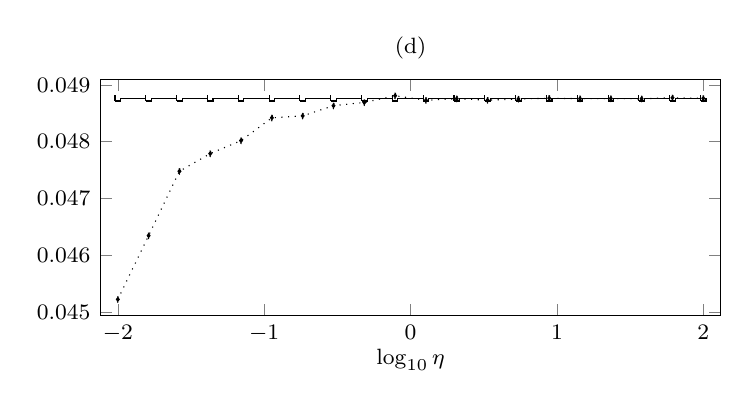
\begin{tikzpicture}
\begin{axis}[
    title={(d)},
    xlabel={$\log_{10}\eta$},
    xmode=log,
    log basis x=10,
    xmin=0.01,
    xmax=100,
    enlarge x limits=0.03,
    xtick={0.01,0.1,1,10,100},
    xticklabels={$-2$, $-1$, $0$, $1$, $2$},
    scaled y ticks=false,
    scale only axis,
    width=0.65\linewidth,
    height=3.0cm,
    mark size=1.0pt,
    font=\footnotesize,
    xlabel style={yshift=1ex},
    title style={yshift=-0.5ex},
    enlarge y limits=0.08,
    ytick distance=0.001,
    yticklabel style={/pgf/number format/fixed,/pgf/number format/precision=3},
]
\addplot[black, solid, mark=none]
coordinates
{(0.01,0.04876645583855118) (0.016237767391887217,0.04876645583855118) (0.02636650898730358,0.04876645583855118) (0.04281332398719394,0.04876645583855118) (0.06951927961775606,0.04876645583855118) (0.11288378916846889,0.04876645583855118) (0.18329807108324356,0.04876645583855118) (0.29763514416313175,0.04876645583855118) (0.4832930238571752,0.04876645583855118) (0.7847599703514611,0.04876645583855118) (1.2742749857031335,0.04876645583855118) (2.06913808111479,0.04876645583855118) (3.359818286283781,0.04876645583855118) (5.455594781168514,0.04876645583855118) (8.858667904100823,0.04876645583855118) (14.38449888287663,0.04876645583855118) (23.357214690901213,0.04876645583855118) (37.92690190732246,0.04876645583855118) (61.584821106602604,0.04876645583855118) (100.0,0.04876645583855118)}
;
\addplot[black, dashed, mark=square*, mark size=1.0pt, mark options={fill=white}]
coordinates
{(0.01,0.04876645583855118) (0.016237767391887217,0.048766455838551194) (0.02636650898730358,0.04876645583855117) (0.04281332398719394,0.048766455838551194) (0.06951927961775606,0.04876645583855117) (0.11288378916846889,0.04876645583855117) (0.18329807108324356,0.048766455838551194) (0.29763514416313175,0.04876645583855117) (0.4832930238571752,0.04876645583855118) (0.7847599703514611,0.048766455838551194) (1.2742749857031335,0.0487664558385512) (2.06913808111479,0.04876645583855117) (3.359818286283781,0.04876645583855117) (5.455594781168514,0.048766455838551166) (8.858667904100823,0.048766455838551166) (14.38449888287663,0.048766455838551166) (23.357214690901213,0.04876645583855113) (37.92690190732246,0.0487664558385512) (61.584821106602604,0.04876645583855117) (100.0,0.048766455838551194)}
;
\addplot[black, dotted, mark=diamond*, mark size=1.0pt]
coordinates
{(0.01,0.04522628871824022) (0.016237767391887217,0.0463486454942992) (0.02636650898730358,0.047480831834152984) (0.04281332398719394,0.04779207087248951) (0.06951927961775606,0.04802044328738652) (0.11288378916846889,0.04842103523171031) (0.18329807108324356,0.0484556297299152) (0.29763514416313175,0.04863420657715559) (0.4832930238571752,0.04869194546628785) (0.7847599703514611,0.048809526686420024) (1.2742749857031335,0.04872986492094675) (2.06913808111479,0.048757462527530805) (3.359818286283781,0.04873211974650815) (5.455594781168514,0.04875220090890722) (8.858667904100823,0.04876577762599834) (14.38449888287663,0.04875808305892399) (23.357214690901213,0.04875987156872306) (37.92690190732246,0.04875658678927084) (61.584821106602604,0.04877379669723203) (100.0,0.04876350040005571)}
;
\end{axis}
\end{tikzpicture}
\end{subfigure}%
\caption{Simulation results for $\beta^{\lambda}$ over the learning-rate grid, using common data sets with $G=100$, $m=5$, and $n=500$.
Panels show (a) coverage of nominal $95\%$ intervals, (b) mean interval width, (c) mean bias, and (d) standard deviation of the estimation error.
Solid line: sandwich Wald benchmark; dashed line with squares: calibrated posterior; dotted line with diamonds: uncalibrated posterior.
The horizontal reference in panel~(a) is $0.95$.
}
\label{fig:random-intercept-exp}
\end{figure}
